\section{Exercise 6}
The following algorithm was used to perform the $LU$ factorization 

\begin{algorithm}[H]
\DontPrintSemicolon
\SetAlgoLined
\KwResult{Factoring matrix $A$ into $L$ and $U$}
\SetKwInOut{Input}{Input}\SetKwInOut{Output}{Output}
\Input{$A$}
\Output{$L$, $U$}
\BlankLine
$L = I(3)$    \;
$U = A $    \;
\BlankLine
    \For{k in range(0, M-1)}{    
    \For{j in range(k+1, M)}{
       L[J,K]      = U[J,K]/U[K,K] \;
       U[J,K:]     = U[J,K:]-L[J,K]*U[K,K:] \;
       U[J,K]      = 0.0
    }    
}
\caption{$LU$ Factorization}
\end{algorithm}

Secondly, we can plot the number of points versus computational time, as
seen in Fig~.(\ref{fig:lu-factorization}), where we see how important it
is to use built in Python packages. 
\begin{figure}[H]
    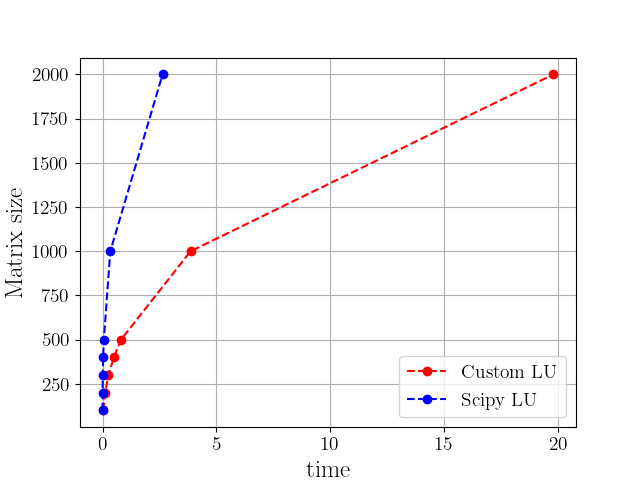
\includegraphics[height=3.0in]{media/exercise-6.png}
    \caption{Performance study of user defined $LU$ factorization tool}
    \label{fig:lu-factorization}
\end{figure}
For an example of the complete code please refer to the Appendix.
